\section{Anexos}
\bigskip
\subsection{TL494}\label{TL494}

El TL494 es un circuito de control de modulación de ancho de pulso a frecuencia constante. La modulación del pulso de salida es lograda comparando la forma de onda triangular entregada por el oscilador interno con cualquiera de las señales de control. Estas señales pueden ser sacadas del circuito del control de tiempo muerto (deadtime control) o del amplificador de error. La entrada de control de tiempo muerto es comparada directamente con una compensación de 120mV (que fija un tiempo muerto por default). El comparador PWM compara la señal de control creada por los amplificadores de error con la triangular. La función del amplificador de error es supervisar la tensión de salida y proporcionar la ganancia suficiente de modo que unos pocos milivolts de error en su entrada causen una señal de control de amplitud suficiente para proporcionar control de modulación del $100\% $. Los amplificadores de error también pueden ser usados para supervisar la corriente de salida y proporcionar la limitación de corriente con la carga.

\subsubsection{Terminales del TL494}

Se procede a detallar las terminales de este integrado tal como se muestran en la Figura~\ref{TL494}.

\begin{figure}[H]
\centering
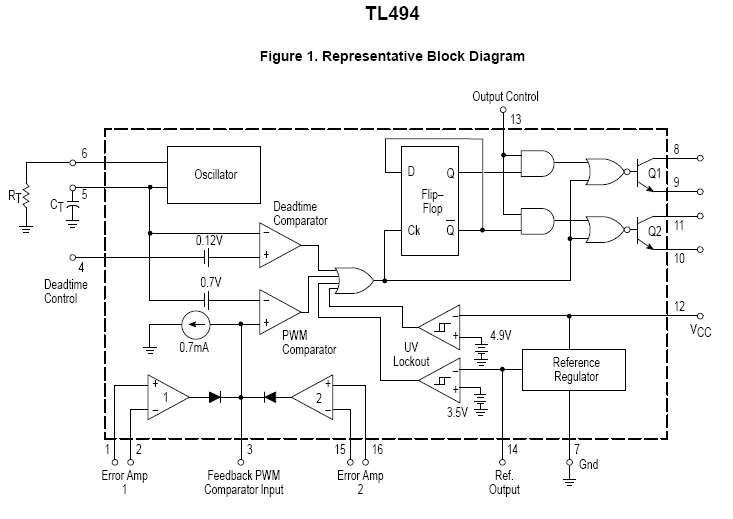
\includegraphics[width=\textwidth]{img/tl494.png}
\caption{Diagrama en bloques del circuito interno del integrado TL494.}
\label{tl494}
\end{figure}

\begin{enumerate}
\item Terminal positivo del comparador 1, utilizado para la realimentación.
\item Terminal negativo del comparador 1, utilizado para la realimentación.
\item Terminal de realimentación del PWM y terminal positivo del comparador PWM. Se utiliza para evitar efectos parásitos.
\item Terminal del circuito de control de tiempo muerto (deadtime control). Se utiliza para evitar efectos parásitos
\item Terminal del oscilador. Para que el oscilador funcione se conecta un capacitor entre terminal y masa.
\item Terminal del oscilador. Para que el oscilador funcione se conecta un resistor entre terminal y masa.
\item Terminal del regulador de referencia. Para que el regulador funcione se conecta este terminal a masa.
\item Terminal de drain del transistor 1. 
\item Terminal de source del transistor 1
\item Terminal de drain del transistor 2
\item Terminal de source del transistor 2
\item Terminal de alimentación del circuito
\item Terminal de salida utilizado como control. Se utiliza para evitar efectos parásitos.
\item  Terminal que brinda la tensión de referencia de 5V del regulador de referencia interno del circuito.
\item Terminal positivo del comparador 2, utilizado para la realimentación.
\item Terminal negativo del comparador 2, utilizado para la realimentación.
\end{enumerate}
